Существенным препятствием распределенного обучения является 
проблема передачи данных и обновление представлений участников об общем состоянии системы.
В секции будут разобраны проблемы и пути решения, включающие ролевые

\begin{figure}[h]
    \centering
    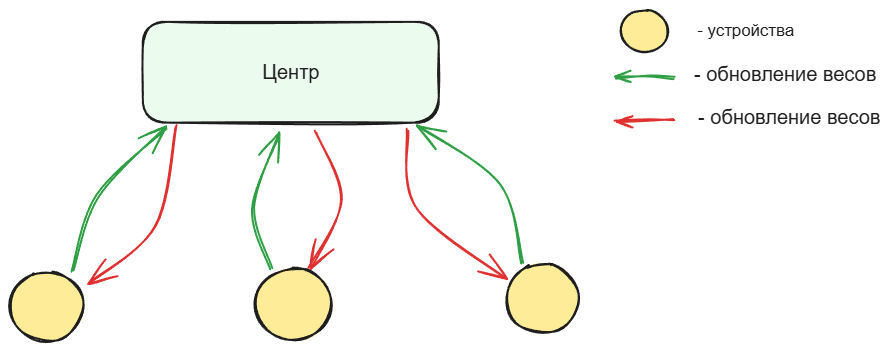
\includegraphics[width=0.5\textwidth]{assets/math/distributed/distributed.excalidraw.png}
    \caption{Распределенное обучение включает }
    \label{distributed}
\end{figure}


Виды распределенного обучения \begin{itemize}
    \item кластерное - единая организация с доверенными узлами
    \item коллаборативное - распределенняя организация
    \item федеративное - на устройствах пользователей  с применением
\end{itemize}

\begin{figure}[h]
    \centering
    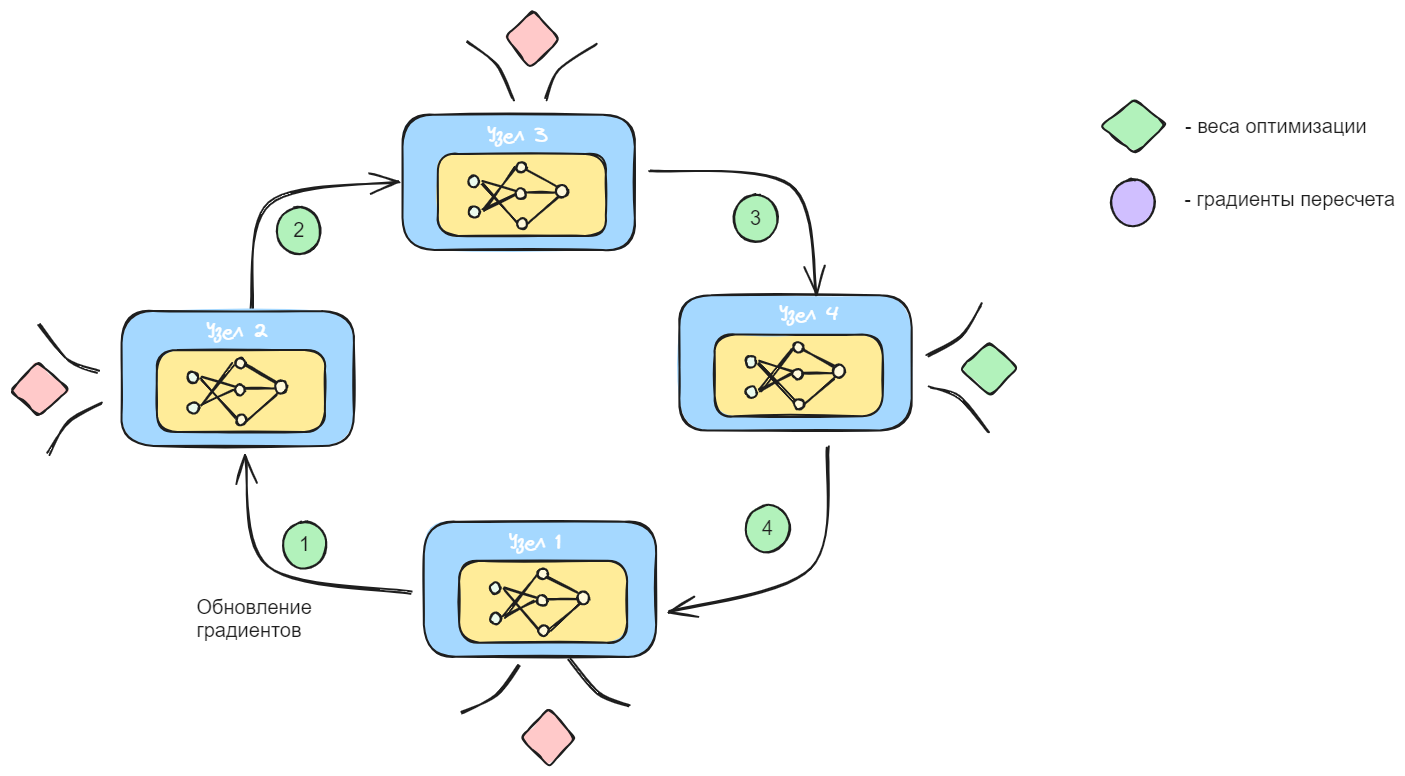
\includegraphics[width=0.5\textwidth]{assets/math/distributed/ring.excalidraw.png}
    \caption{Одной из распространенных архитектур взаимодействия является кольцевая.}
    \label{ring}
\end{figure}

Ключевыми вопросами для разработки алгоритма являются определение \begin{itemize}
    \item число пересчетов на вычислительных узлах $N$
    \item число коммуникаций при вычислениях $K$
    \item степень компрессии при коммуникациях $\beta$ 
\end{itemize}
    
\textit{Опредление} \textbf{Несмещенной компрессией} называется компрессия $\Pi$ со свойствами \begin{itemize}
    \item $\mathbb{E}[\Pi(x)] = x$
    \item $\mathbb{E}[\|\Pi(x)\|^2_2] \le \omega \| x \|^2_2$, где $\omega \ge 1$
\end{itemize}

Определим современные подходы к компрессии в постановке распределенных систем. 

\textit{Опредление} \textbf{Случайной спарсификацией} \cite{richtarik2016parallel}называется оператор, выбирающий из вектора компоненты по правилу
\begin{equation}
    \text{Rankd}(x) = \frac{d}{k} \sum_{i \in S} x_i e_i,
\end{equation}
где $i$ - случайно выбранные компоненты из базиса.

\textit{Определение} \textbf{Трехуровневая} $\mathcal{l}_2$ квантизация задается оператором
$Q(x)=\|x\|_2 \text{sign}(x)\xi_i$, $i=1,\dots,d$  и $xi_i$ -бернулевская случайная величина с параметром
определяемым вкладом компоненты в модуль $\frac{|x_i|}{\|x\|_2}$.

\textit{Определение}
Пусть $\text{round}_\nu^-$ оператор округляющий число до ближайшей степени $\nu \in \mathcal{N}$ снизу, 
$\text{round}_\nu^+$ анологичный оператор для округления в большую сторону. Тогда \textbf{Натуральная компрессия} задается оператором
\begin{equation}
    \text{Nat}(x)_i = \left\{\begin{array}{c}
        \text{round}_2^-(x_i), \ \text{c вероятностью} p=\frac{x_i - \text{round}_2^-(x)}{\text{round}_2^+(x)-\text{round}_2^-(x)} \\
        \text{round}_2^+(x_i) \\
    \end{array}\right.    
\end{equation}

\textit{Теорема} Если все функции $f_m$ являются $\mu$-сильно выпуклыми
и имеют $L$-Липшицев градиент, тогда при шаге $\eta \le L^{-1} (\frac{2 \omega}{M}+1)^{-1}$:
\begin{equation}
    \mathcal{O}\left(
        (1-\gamma \mu)^K \|x_0 -x^*\|^2 + \frac{1}{K} \frac{2 \omega}{\mu M^2} \sum_{m=1}^M \| \nabla f_m(x^*) \|^2
    \right)
\end{equation}

Локальный градиентный спуск
\cite{karimireddy2020scaffold}

\cite{stich2019unified}

\cite{szlendak2021permutation}

Достижение консенсуса выполняется через алгоритмы распределенных вычислений. 

\textit{Определение}\textbf{Консенсус} является результатом достижения согласованного состояния между несколькими независимыми 
процессами или узлами в системе, которые могут взаимодействовать друг с другом. 

Для достижения консесуса необходимо выполнить условия \begin{enumerate}
    \item корректности: $\forall i \in \{1, \ldots, n\}, \text{если } \text{input}(N_i) = v, \text{ то } \forall j \in \{1, \ldots, n\}, \text{output}(N_j) = v$.
     Все узлы начинают с одним и тем же начальным значением v, то любое значение, принятое в результате выполнения протокола консенсуса, должно быть равно \( v \).
    \item единогласие: $\forall i, j \in \{1, \ldots, n\}, \text{если } \text{output}(N_i) = v, \text{ то } \text{output}(N_j) = v$.
     Если один узел завершает протокол с некоторым значением \( v \), то все другие узлы, которые также завершили протокол, должны иметь то же самое значение \( v \).
    \item завершение:$\forall i \in \{1, \ldots, n\}, \text{ узел } N_i$ 
    завершает выполнение протокола в конечное время.
\end{enumerate}

Наиболее полулярными алгоритмами достижения конcенсуса являются Raft \cite{lamport2019time} и Paxos \cite{pease1980reaching}. Методы
предлагают разделение на роли.

